\documentclass[12pt]{article}

\usepackage{sbc-template}
\usepackage{graphicx,url}
\usepackage[brazil]{babel}   
\usepackage[utf8]{inputenc}  
    
\sloppy

\title{Recuperação de Informação -- Relatório do Trabalho Prático 1}
\author{Danilo Ferreira e Silva\inst{1}}
\address{Departamento de Ciência da Computação -- UFMG
  \email{danilofes@gmail.com}
}

\begin{document} 

\maketitle
     
\begin{resumo} 
  Este relatório descreve o desenvolvimento do trabalho prático 1, proposto na 
  disciplina Recuperação de Informação. O trabalho consistiu da implementação de um
  indexador e processador de consultas simples, aplicando o conhecimento aprendido em
  aula. Experimentos realizados no sistema desenvolvido mostraram que ele é capaz de gerar
  índices, na forma de listas invertidas, para coleções da ordem de 1 milhão de
  documentos em aproximadamente uma hora.
\end{resumo}


\section{Introdução}

Falar alguma bobagem.


\section{Arquitetura do sistema} \label{sec:firstpage}

O sistema foi construído na linguagem C++, conforme especificado, e é constituido de 
dois executáveis. O primeiro deles é o indexador da coleção de documentos, que gera 
um arquivo de listas invertidas ao final do processamento.
O segundo é o processador de consultas, que usa o arquivo gerado pelo
indexador para responder a consultas do usuário de forma interativa, via linha de
comando.


\subsection{Módulos e dependências}

Na figura~\ref{fig:modules} são apresentados os módulos e dependências entre eles.

\begin{figure}[ht]
\centering
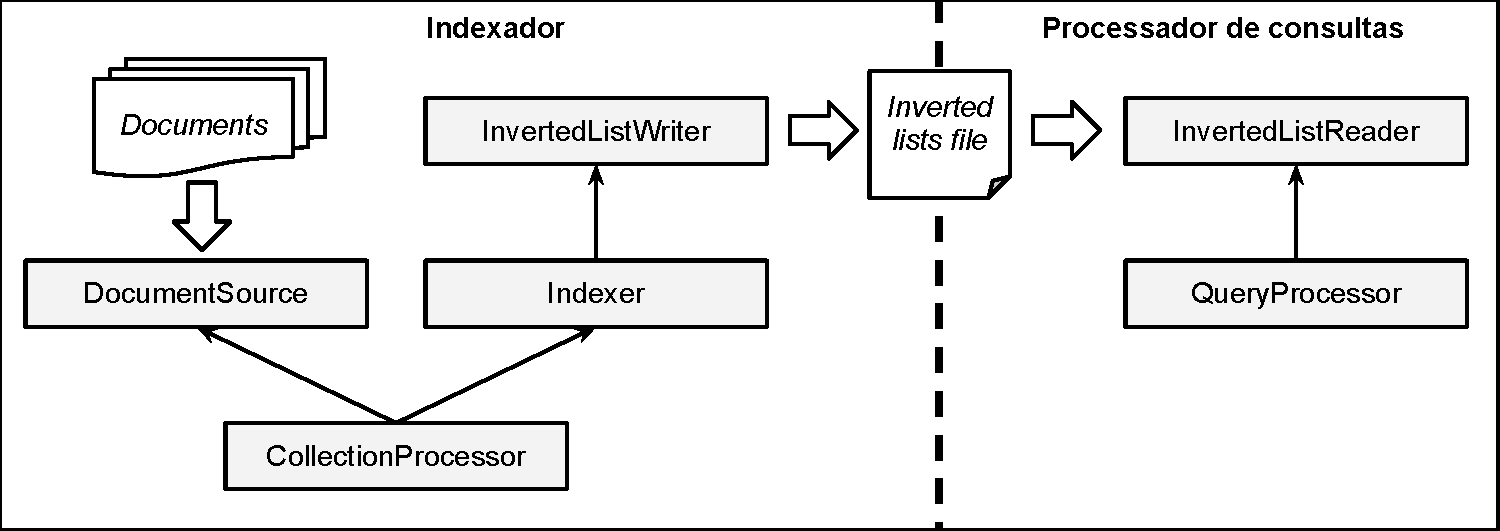
\includegraphics[width=1\textwidth]{modules.pdf}
\caption{Diagrama de dependências de módulos do sistema}
\label{fig:modules}
\end{figure}

\begin{description}
\item[DocumentSource] Abstração que representa uma fonte de documentos, identificados por uma URL e cujo conteúdo é uma sequência de caracteres. A implementação lê os documentos usando a RICPlib.
\item[CollectionProcessor] Módulo principal que lê um conjunto de documentos fornecidos pelo \emph{DocumentSource}, transforma-os em uma sequência de termos e alimenta o \emph{Indexer}.
\item[Indexer] Recebe um conjunto de termos dos documentos e faz a indexação. Ao final escreve as listas invertidas usando o \emph{InvertedListWriter}.
\item[InvertedListWriter] Escreve o arquivo de listas invertidas.
\item[InvertedListReader] Lê o arquivo de listas invertidas.
\item[QueryProcessor] Processa uma consulta e devolve os resultados.
\end{description}


\subsection{Dependência a bibliotecas de terceiros}

O sistema foi contruído usando a API padrão C++11. Além disso, foram utilizadas as bibliotecas listadas a seguir.

\begin{description}
\item[RICPlib] Biblioteca fornecida na especificação para ler a coleção de documentos comprimida.
\item[zlib] Dependência indireta induzida pela RICPlib.
\item[htmlcxx] Parser de documentos HTML.
\item[gmock] Biblioteca para criação de \textit{mock objects} (usada apenas em testes unitários).
\end{description}


\section{Algoritmos e estruturas de dados utilizados}

O processo de indexação pode ser subdividido nas três etapas descritas abaixo:
\begin{enumerate}
\item Leitura dos documentos e escrita das triplas no arquivo temporário.
\item Ordenação das triplas, subdivididas em vários blocos de acordo com o tamanho do buffer.
\item \emph{Merge} dos blocos, e geração das listas invertidas.
\end{enumerate}

Na etapa 1, a principal estrutura de dados envolvida é o vocabulário. Ele é representado internamente por uma tabela \emph{hash}, onde a chave é o próprio termo. Cada entrada da mesma também contém um identificador numérico atribuído ao termo e um contador de ocorrências do termo em documentos. Adicionalmente, ao processar um documento, é criado uma estrutura para guardar o vocabulário local, tembém usando uma tabela \emph{hash}. Nesta a chave é o identificador do termo, e a entrada é um contador de frequência do termo no documento.

Portanto, para cada termo de cada documento, consulta-se primeiro o vocabulário para obter o identificador do termo (ou criar um novo). Em seguida é consultado o vocabulário local, para atualizar a frequência do mesmo no documento. Ambas as operações são $O(1)$, portanto a primeira etapa tem custo de tempo linear com relação ao número total de termos. O custo de memória é proporcional ao número de termos distintos.


\subsection{Ordenação externa das triplas}

As etapas 2 e 3 do algoritmo são na verdade uma ordenação externa. Para que seja viável indexar uma grande coleção de documentos, o índice não pode ser mantido todo em memória. Isso torna necessário o uso da ordenação externa.

A etapa 2 consiste na primeira etapa da ordenação das triplas no arquivo invertido, onde o conjunto de triplas são divididos em blocos menores de tamanho constante $k$. Para cada um desses blocos, é feita uma ordenação em memória usando o algoritmo \emph{heapsort}, cujo custo é $O(n \log{n})$.

Consideranto $T$ o número total de triplas, o custo dessa etapa é aproximadamente: 
$$\lceil T/k \rceil k \log{k}$$
que é linear para efeitos práticos, pois $\log{k}$ é uma constante.

Finalmente na etapa 3, é feita uma intercalação de múltiplos caminhos nos $R = \lceil T/k \rceil$ blocos ordenados em disco. Para isso é utilizado um \emph{heap} de tamanho $R$. Para cada tripla retirada do mesmo, ele é reconstruído com custo logaritmico. O custo total pode ser aproximado como:
$$T \log{\lceil T/k \rceil}$$



\section{Avaliação}

Para avaliar o desempenho do sistema, foram executados experimentos com tamanhos variados de coleções de documento, bem como com a coleção completa fornecida para testes.


\begin{table}[ht]
\centering
\caption{Tempo de execução em segundos para entradas de tamanho variado}
\label{tab:exec_time_collection}
\begin{tabular}{rrrrr}
Documentos & Etapa 1 & Etapa 2 & Etapa 3 & Total \\ \hline
50000      & 80      & 34      & 23      & 234   \\
100000     & ~       & ~       & ~       & ~     \\
150000     & ~       & ~       & ~       & ~     \\
200000     & ~       & ~       & ~       & ~     \\
1000000    & ~       & ~       & ~       & ~     \\
\end{tabular}
\end{table}


\begin{table}[ht]
\centering
\caption{Tempo de execução em segundos para \emph{buffer} de tamanho variado}
\label{tab:exec_time_buffer}
\begin{tabular}{rrrrr}
Documentos & Etapa 1 & Etapa 2 & Etapa 3 & Total \\ \hline
50000      & 80      & 34      & 23      & 234   \\
100000     & ~       & ~       & ~       & ~     \\
150000     & ~       & ~       & ~       & ~     \\
200000     & ~       & ~       & ~       & ~     \\
1000000    & ~       & ~       & ~       & ~     \\
\end{tabular}
\end{table}




\section{References}

Bibliographic references must be unambiguous and uniform.  We recommend giving
the author names references in brackets, e.g. \cite{knuth:84},
\cite{boulic:91}, and \cite{smith:99}.


\bibliographystyle{sbc}
\bibliography{tc}

\end{document}
